\section{Bevezetés}

Napjainkban egyre inkább terjednek el a különféle drónok, távirányítással vagy
akár önálló módon repülő többrotoros kopterek formájában. Számos nagyobb gyártó
(például DJI, Parrot) is kínál a fogyasztói piacon készen megvásárolható
termékeket, továbbá számtalan lelkes ember áll neki otthon kísérletezni ilyesmi
szerkezetek építésével.

Az ELTE Biológiai Fizika Tanszékével szoros együttműködésben a CollMot kft.
rendelkezik körülbelül 40 saját építésű kopterrel, amelyeken az alacsonyabb
szintű motorvezérlő pilótaprogram felett belső fejlesztésű rendszerük fut.

A szóban forgó drónok felhasználása igencsak változatos. Kutatási oldalról
például különböző tudományos szimulációk tesztelésére is alkalmasak, mint
akár madarak vagy halak viselkedésének vizsgálata egyszerű fizikai törvényeken
alapuló rajzási modellek evolúciójának segítségével. Ezen felül szolgálhatnak
továbbá látványelemként is egy előre betáplált koreográfia útvonalának
végigrepülése közben LED lámpájuk fényerejét és színét változtatva.

\begin{figure}[h!]
  \center
  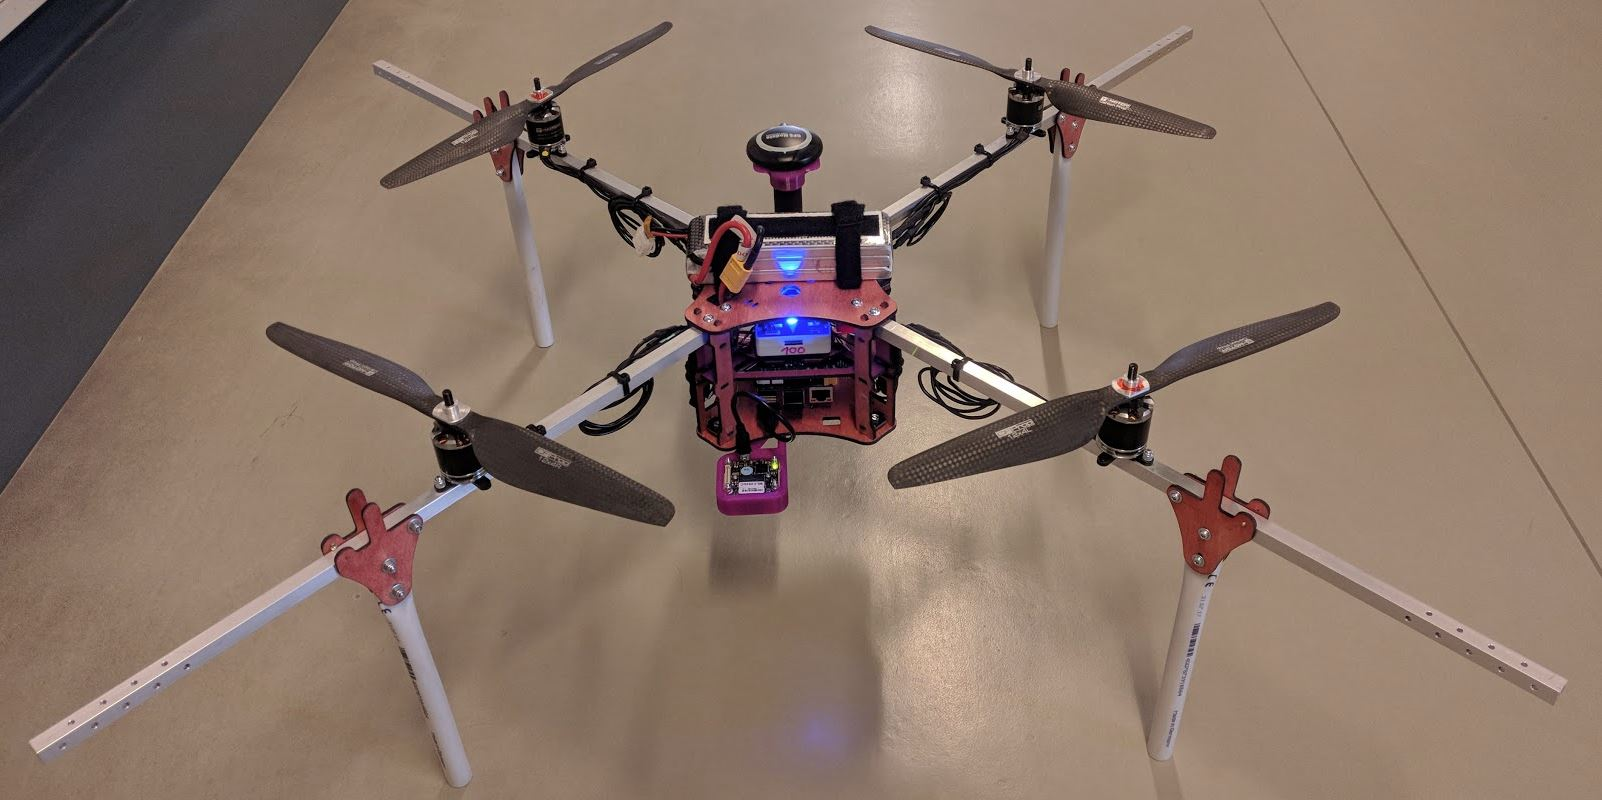
\includegraphics[width=0.8\textwidth]{drone.jpg}
  \caption{Fénykép a fent említett kopterek egy példányáról}
  \label{fig:drone}
\end{figure}

A FlockWave szoftver ötlete az ezen drónok monitorozására és vezérlésére készült
régebbi GroundControl nevű parancssori eszköz (lásd \ref{fig:groundcontrol}.
ábra) grafikus megjelenítéssel rendelkező megoldásra történő leváltásának
céljával fogalmazódott meg.

% TODO: Két mondatba?

Léteznek már kész, elérhető szoftverek hasonló célokra, azonban a kereskedelmi
drónokhoz való, gyártók által mellékelt programok általában nem flották, hanem
leginkább csak egy-egy drón kezelésére alkalmasak, ráadásul zártak, tehát csak
a gyártó saját termékeivel működnek.

Természetesen nem új gondolat a több kopter kezelésére is képes általános
vezérlési felület sem. Ilyen az UgCS nevű program (https://www.ugcs.com), amely
számos protokollt támogat, így sok gyártó eszközeivel képes kommunikálni,
ráadásul elméletileg korlátlan számú drónt tud kezelni, azonban zárt, és így a
piacon lévő egyeduralmának köszönhetően nagyon drága.

Nyílt forráskódú kezdeményezés említésének céljából érdemes a QGroundControl-t
(http://qgroundcontrol.com/) kiemelni, ami egy nagyon sokoldalú program,
azonban sajnos egyidejűleg csak egy kopter kezelésére képes.

\begin{figure}[H]
  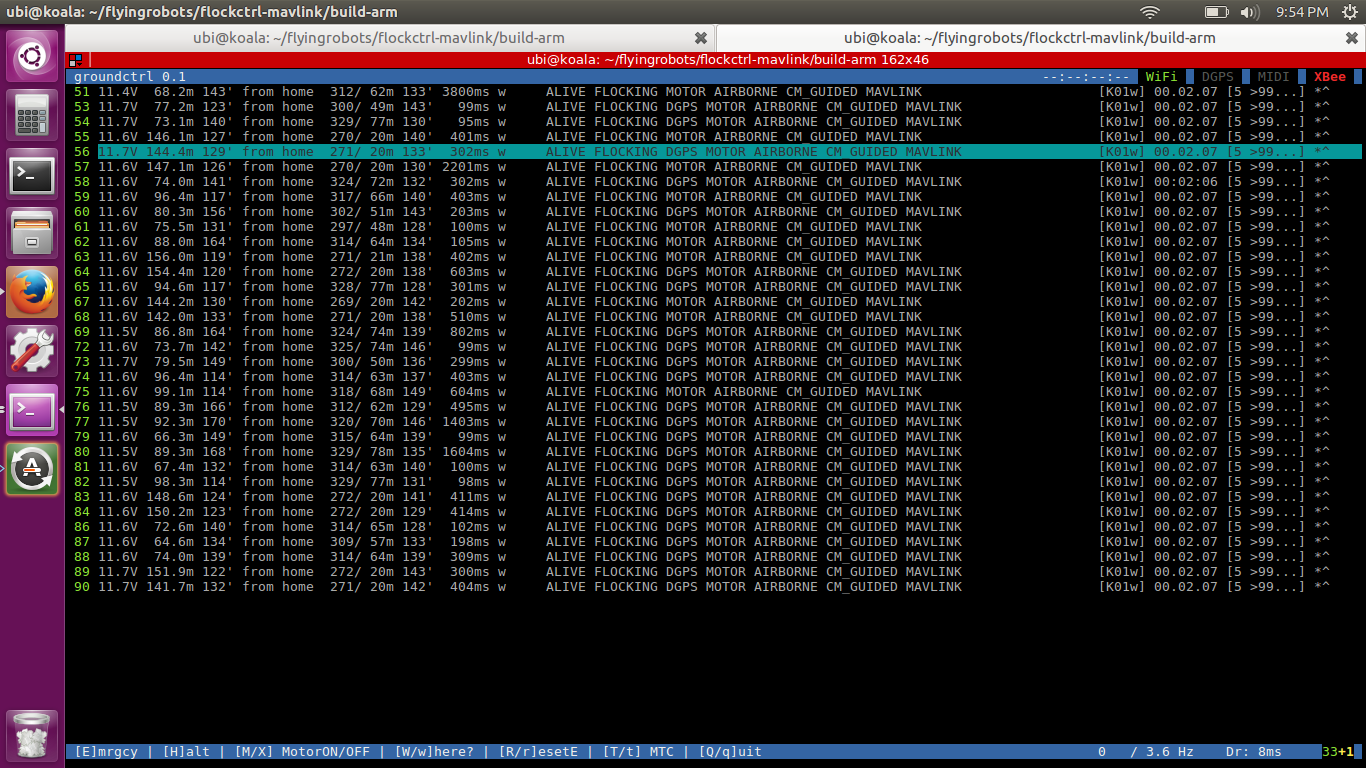
\includegraphics[width=\textwidth]{groundcontrol.png}
  \caption{Képernyőfotó a lecserélésre szánt régi karakteres kezelőfelületről}
  \label{fig:groundcontrol}
\end{figure}

\noindent A FlockWave szoftver ötletének a megvalósítási folyamatába
kapcsolódtam be még abban a kezdeti szakaszban, amikor a program körülbelül csak
a drónok pozícióját tartalmazó szerverről érkező csomagok feldolgozására és az
ezekből származó adatok alapján történő térképen való megjelenítésére volt
alkalmas. Ekkor lett a feladatom a rendszer további funkciókkal történő
ellátása. Ezek közül néhányat mutatok be kiemelve ebben a szakdolgozatban.
